\documentclass{standalone}

\usepackage{tikz}
\usetikzlibrary{automata, positioning, arrows, calc}

\tikzset{
	->,  % makes the edges directed
	>=stealth, % makes the arrow heads bold
	shorten >=2pt, shorten <=2pt, % shorten the arrow
	node distance=3cm, % specifies the minimum distance between two nodes. Change if n
	every state/.style={draw=blue!55,very thick,fill=blue!20}, % sets the properties for each ’state’ n
	initial text=$ $, % sets the text that appears on the start arrow
 }

\begin{document}
	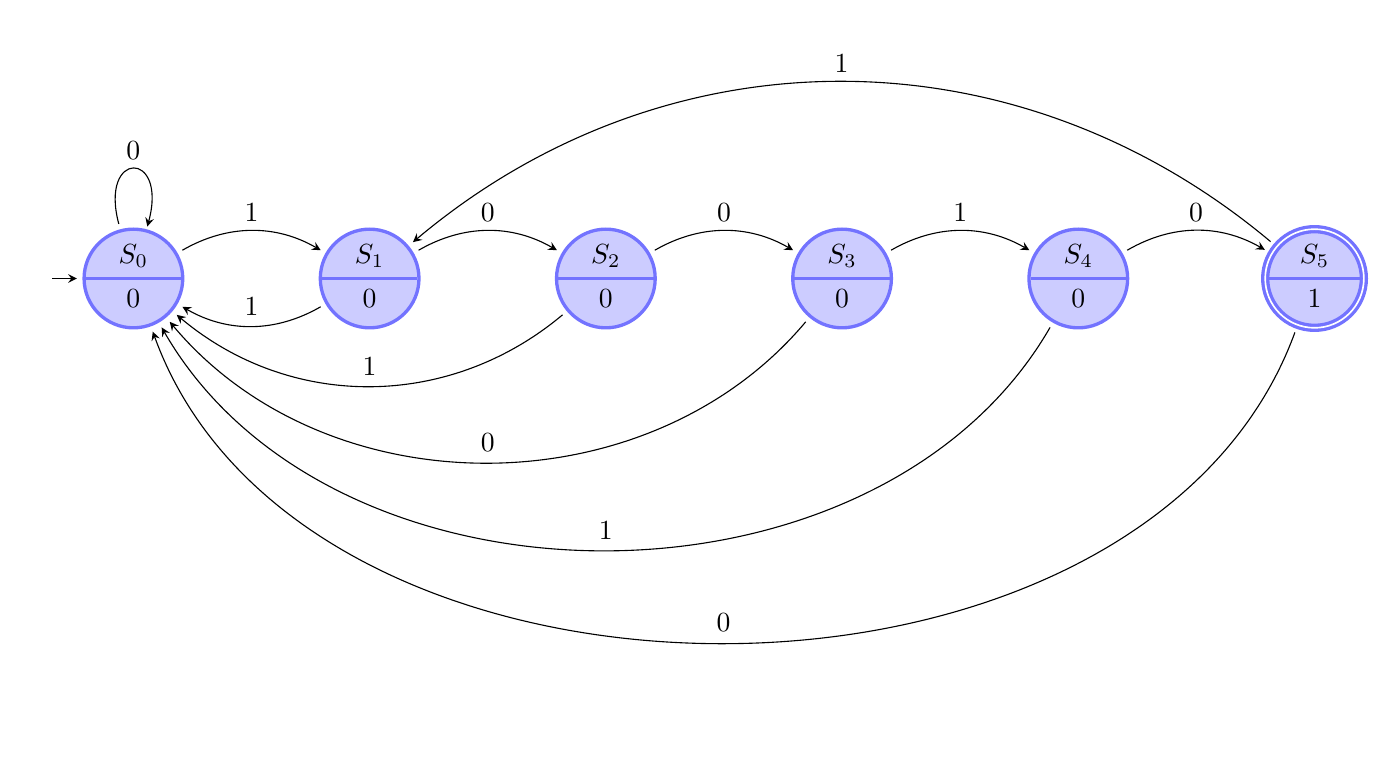
\begin{tikzpicture}
		\node[state with output, initial] (s0) {$S_0$ \nodepart{lower} $0$};
		\node[state with output, right of=s0] (s1) {$S_1$ \nodepart{lower} $0$};
		\node[state with output, right of=s1] (s2) {$S_2$ \nodepart{lower} $0$};
		\node[state with output, right of=s2] (s3) {$S_3$ \nodepart{lower} $0$};
		\node[state with output, right of=s3] (s4) {$S_4$ \nodepart{lower} $0$};
		\node[state with output, accepting, right of=s4] (s5) {$S_5$ \nodepart{lower} $1$};
		
		\draw (s0) edge[loop above] node{$0$} (s0)
			  (s0) edge[bend left] node[above]{$1$} (s1)
			  %
			  (s1) edge[bend left] node[above]{$0$} (s2)
			  (s1) edge[bend left] node[above]{$1$} (s0)
			  %
			  (s2) edge[bend left] node[above]{$0$} (s3)
			  (s2) edge[bend left=40] node[above]{$1$} (s0)
			  %
			  (s3) edge[bend left=50] node[above]{$0$} (s0)
			  (s3) edge[bend left] node[above]{$1$} (s4)
			  %
			  (s4) edge[bend left] node[above]{$0$} (s5)
			  (s4) edge[bend left=60] node[above]{$1$} (s0)
			  %
			  (s5) edge[bend right=40] node[above]{$1$} (s1)
			  (s5) edge[bend left=70] node[above]{$0$} (s0)
		;
	\end{tikzpicture}
\end{document}